\section{Layout & Control Erweitert}
\subsection{Benutzerführung}
Die höchste Klasse jeder XAML App ist die \code{System.Windows.Application}. Beinhaltet:
    \begin{description}
        \item[Current] Property (Singelton) bietet statischen Zugriff auf das Application Objekt
        \item[MainWindow] das Zugriff auf das Hauptfenster bietet
        \item[ShutdownMode] welche das Verhalten beim Programmende definiert
    \end{description}

\paragraph{Current} Das Application Objekt ist als Singelton implentieret. Um es innerhalb der App zu verwenden, muss es oft gecastet werden.
\begin{lstlisting}
public App MyApp => Application.Current as App;
\end{lstlisting}
\paragraph{ShutdownMode} Der ShutdownMode definiert das Verhalten der App beim beenden, davon gibt es 3.
\begin{itemize}
\item \code{OnLastWindowClose}: Dies ist das Standardverhalten, die App beendet sich, sobald das letzte Fenster geschlossen wurde
\item \code{OnMainWindowClose}: Die App wird beendet sobald das Hauptfenster geschlossen wird
\item \code{OnExplicitShutdown}: Die App wird erst beendet, wenn die \code{Shutdown()} Methode aufgerufen wurde.
\end{itemize}
\paragraph{StartupUri} Dies ist der Name der UI Ressource, die beim Start angezeigt werden soll, es ist normalerweise ein \verb+Window+

\paragraph{Startup}

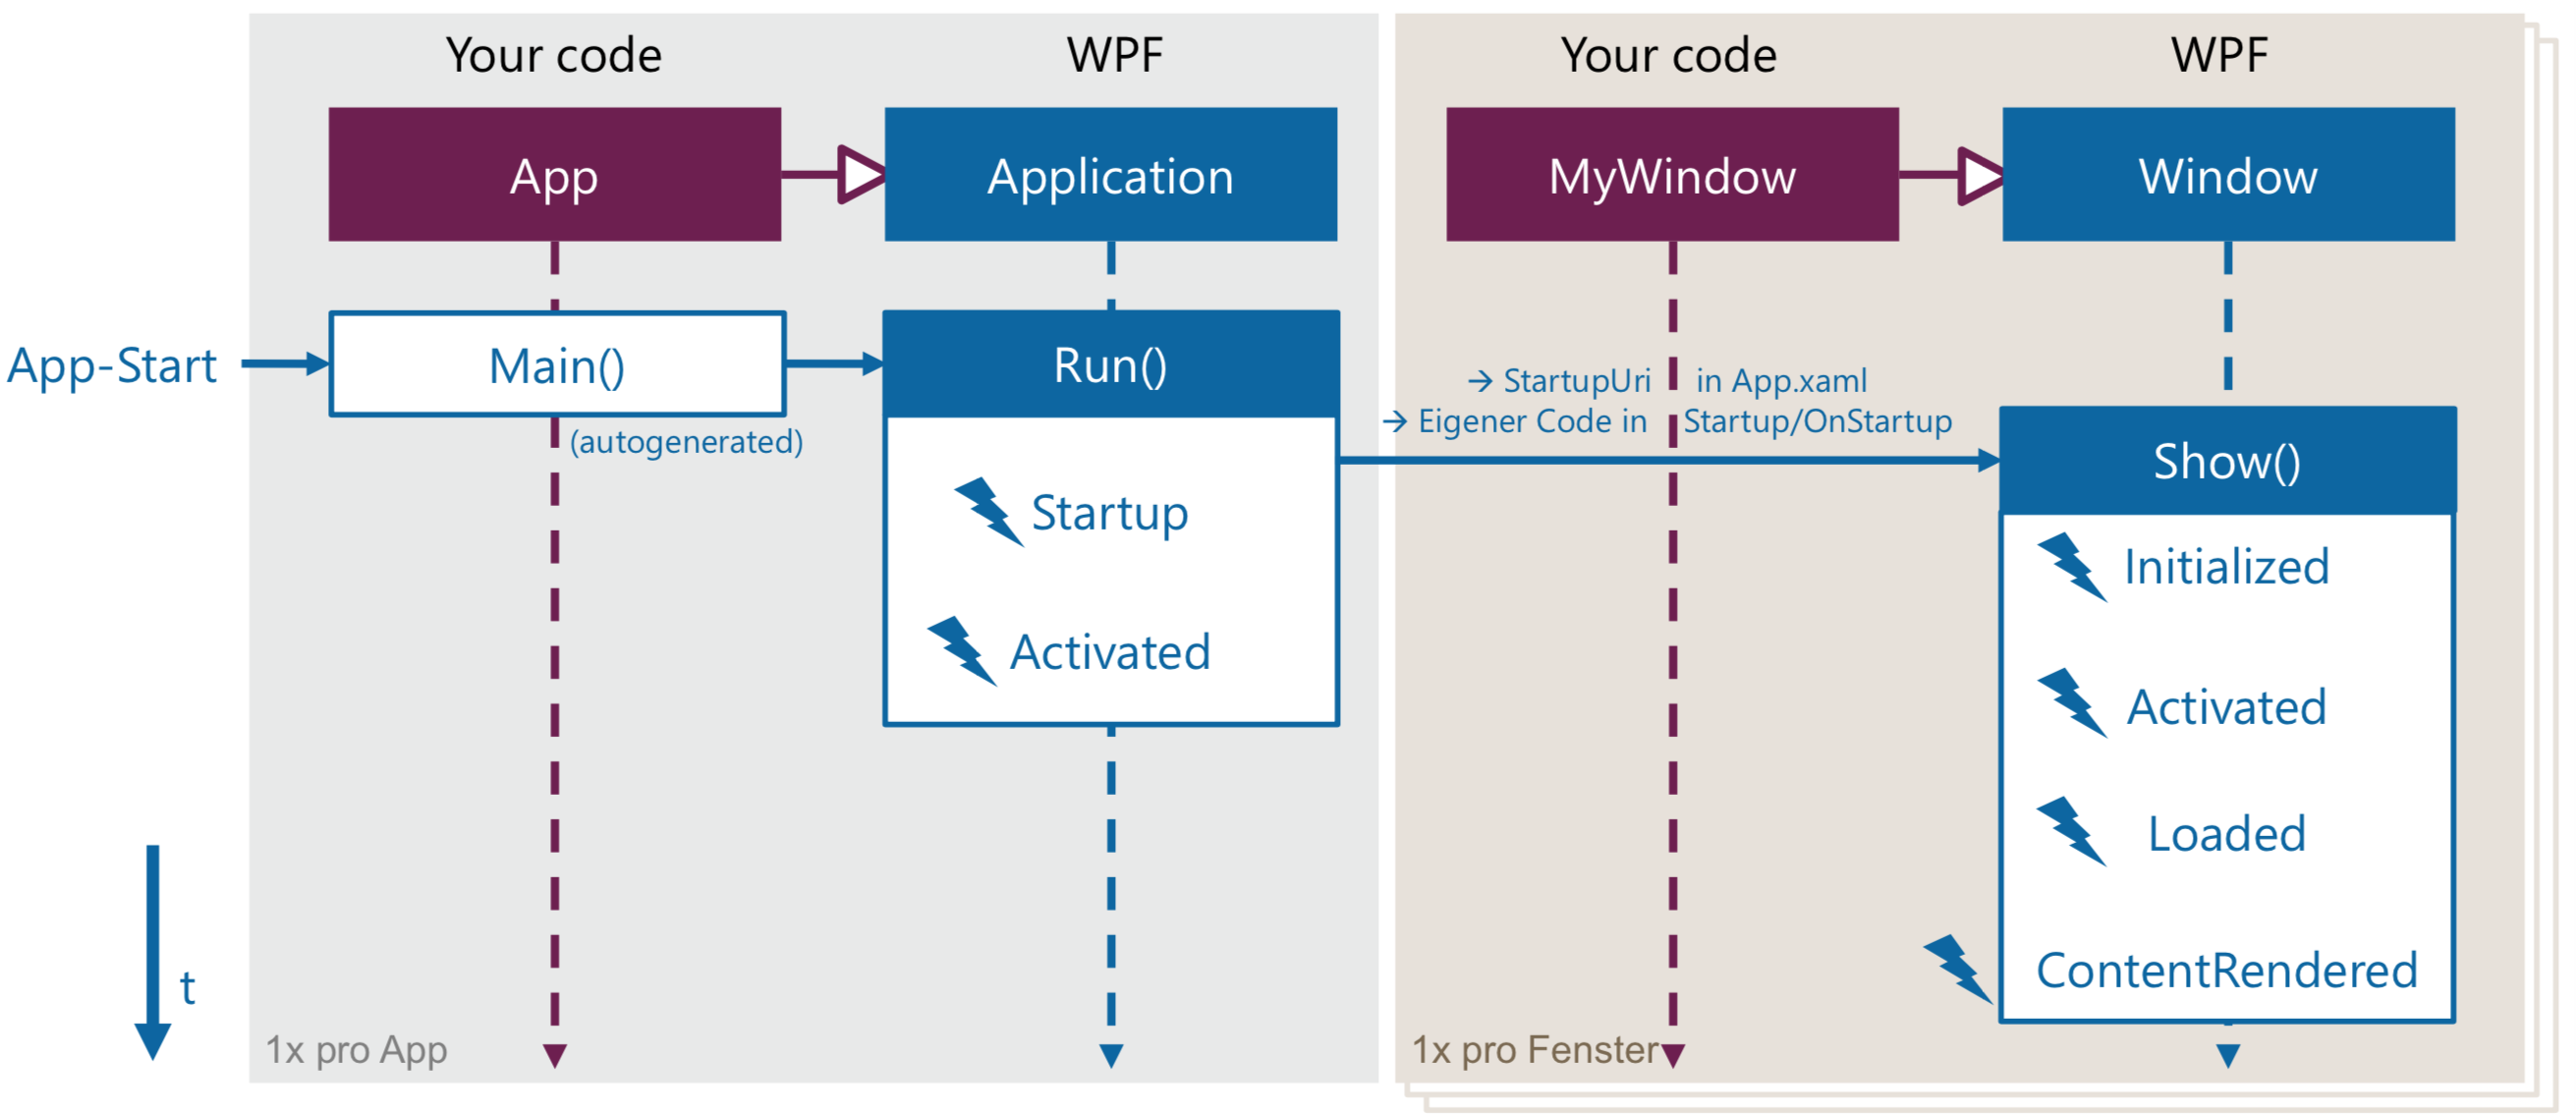
\includegraphics[scale=0.13]{startup.png}

\paragraph{Windows} Das \code{Windows} Property ist eine Liste aller instanziierter Fenster (Window-Objekte) innerhalb der App.
\paragraph{Application-Klasse Methoden} Die \verb+LoadComponent+ Methode lädt eine XAML-Ressource. Der Rückgabetyp muss in den korrekten Typ gecastet werden.
\begin{lstlisting}
public static object LoadComponent(Uri uri)
\end{lstlisting}
Die \verb+FindResouce+ Methode, sucht eine Ressource mit dem angegeben Namen. Es durchsucht App-Ressourcen und System-Ressourcen. Der Rückgabetyp muss ebenfalls in den korrekten Typ gecastet werden.
\begin{lstlisting}
public object FindResource(object resourceKey)
\end{lstlisting}
Die \verb+Shutdown+ Methode beendet die App und gibt optional einen mitgegebenen Exit Code ans System zurück.
\begin{lstlisting}
public void Shutdown([int exitCode])
\end{lstlisting}
\paragraph{Application-Klasse Events}
\begin{itemize}
\item \verb+Activated+: Die App wurde aktivitert (in den Vordergrund geholt)
\item \verb+Deactivated+: Die App wurde deaktiviert
\item \verb+DispatcherUnhandledException+: Eine nicht gefangene Exception ist aufgetreten
\item \verb+Exit+: Die App wird gleich beendet
\item \verb+FragmentNavitation+: Es wurde zu einem bestimmten \verb+NavigationWindow+/\verb+Frame+ navigiert
\item \verb+LoadCompleted+: Aktuelles \verb+NavigationWindow+/\verb+Frame+ wurde vollständig geladen
\item \verb+Navigated+: Aktuelles \verb+NavigationWindow+/\verb+Frame+ wurde gefunden
\item \verb+Navigating+: Navigation zu einem \verb+NavigationWindow+/\verb+Frame+  wurde angefordert
\item \verb+NavigationFailed+: Navigation zu einem \verb+NavigationWindow+/\verb+Frame+ ist fehlgeschlagen
\item \verb+NavigationProgress+: Statusinformation zum Downloadstatus bei Internet-Ressourcen
\item \verb+NavigationStopped+: Ladevorgang des Inhalts der \verb+NavigationWindow+/\verb+Frame+ wurde gestoppt
\item \verb+SessionEnding+: Windows Session wird beendet
\item \verb+Startup+: Die App startet gerade
\end{itemize}


\paragraph{SplashScreen} 
\begin{lstlisting}
private void App_OnStartup(object sender, StartupEventArgs e)
{
    var screen = new SplashScreen("media/splash.png");
    screen.Show(true);
}
\end{lstlisting}
\begin{lstlisting}
//App.xaml.cs
private void App_OnStartup(object sender, StartupEventArgs e)
{
    var screen = new SplashScreen("media/splash.png");
    screen.Show(true); // in den Folien steht false
    Thread.Sleep(2000);
    screen.Close(TimeSPan.FromMilliseconds(500));
}
\end{lstlisting}


\subsection{Window Klasse}
Die \verb+Window+ Klasse beschreibt ein Fenster. Sie ist abgeleitet von \verb+ContentControl+ und erlaubt genau 1 Child Element (\verb+LayoutContainer+).
\begin{itemize}
\item \verb+Icon+: Dieses Property beinhaltet eine ICO-Datei, die als Fenster Icon verwendet wird (Ausführbaren Datei und Fensterttitel)
\item \verb+ShowInTaskBar+: Ein Property das angibt, ob das Fenster in der Taskleite angezeigt wird
\item \verb+Topmost+: Zeigt Fenster über allen andern Fenstern der Anwendung an
\item \verb+SizeToContent+: Legt fest, ob die Grösse eines Fensters automatisch an die Grösse des Inhalts angepasst wird.
    \subitem \verb+Manual+: Fenstergrösse anhand Width/Height Angabe(Standart)
    \subitem \verb+Height+: Höhe wird automatisch anhand des Inhalts festgelegt
    \subitem \verb+Width+: Breite wird automatisch anhand des Inhalts festgelegt
    \subitem \verb+WidthAndHeight+: Breite und Höhe werden automatisch anhand des Inhalts festgelegt
\item \verb+ResizeMode+: Gibt an, wie sich die Fenstergrösse ändern darf. Je nach Einstellung werden zusätzlich die Schaltflächen Minimieren/Maximieren im Fenstertitel angezeigt
    \subitem \verb+NoResize+: Fenstergrösse nicht änderbar
    \subitem \verb+CanMinimize+: Fenster kann minimiert und wiederhergestellt werden
    \subitem \verb+CanResize+: Fenstergrösse kann frei verändert werden (Standard)
    \subitem \verb+CanResizeWithGrip+: Wie \verb+CanResize+ aber mit zusätzlichem Resize Grip unten rechts im Fenster
\item \verb+WindowsStartupLocation+: Legt die Postition beim Start fest
    \subitem \verb+CenterOwner+: Fenster wird in Mitte des aufrufenden angezeigt
    \subitem \verb+CenterScreen+: Fenster wird in der Mitte des Bildschirm angezeigt
    \subitem \verb+Manual+: Position wird durch Left/Top Angabe bestimmt (Standart)
\item \verb+WindowState+: Beschreibt die Fensterzustände (Normal, Minimized, Maximized)
\item \verb+WindowStyle+: Gibt den Rahmentyp des Fensters an:
    \subitem \verb+None+: Nur das Client Area ist sichtbar
    \subitem \verb+SingleBorderWindow+: Fenster mit einfachem (dünnem) Rahmen
    \subitem \verb+ThreeDBorderWindow+: Fenster mit 3D Rahmen
    \subitem \verb+ToolWindow+: Verankertes Tool-Fenster
\end{itemize}
\paragraph{Window-Klasse Methoden}
\begin{itemize}
\item \verb+Activate+: Fenster aktivieren
\item \verb+Close+: Fenster schliessen
\item \verb+DragMove+: Ermöglich das Verschieben des Fensters, falls die linke Maustaste gedrückt ist
\item \verb+GetWindow+: Statische Methode, ruft das Root-Window Objekt zum Control ab (DI)
\item \verb+Hide+: Macht das Fenster unsichtbar
\item \verb+Show+: Zeigt das Fenster an
\item \verb+ShowDialog+: Zeigt das Fenster an und blockiert, bis das Fenster geschlossen wird
\end{itemize}
\paragraph{Window-Klasse Events}
\begin{itemize}
\item \verb+Activated+: Fenster wurde aktiviert
\item \verb+Closed+: Fenster wurde geschlossen
\item \verb+Closing+: Fenster wird gleich geschlossen
\item \verb+ContentRendered+: Fensterinhalt wurde gezeichnet
\item \verb+Deactivated+: Fenster wurde deaktiviert
\item \verb+LocationChanged+: Position des Fensters wurde geändert
\item \verb+StateChanged+: WindowState hat geändert
\end{itemize}
\subsection{Mehrere Fenster}
In WPF ist es möglich mehrere Fenster zu definieren. Diese können zB mit einem ButtonClick angezeigt werden
\begin{description}
\item[.Show()-Methode] zeigt ein Fenster an (Mehrfensterbetrieb) (bei Android nicht möglich)
\item[.ShowDialog()-Methode] zeigt blockierend eine neues Fenster an (siehe nächste subsection)
\end{description}

\subsection{Dialogfenster} 
\begin{itemize}
    \item Dialogfenster dienen zum Abruf von Daten und sind meist Modal (blockierend).
    \item Ein Dialogfenster wird mit der Methode \verb+ShowDialog+ angezeigt. 
    \item Wird Property \code{DialogResult} gesetzt, wird das Dialogfenster automatisch geschlossen
\end{itemize}

\begin{lstlisting}[language=xml]
<Button Content="Cancel" IsCancel="true" />
<Button Name="OkButton" Content="OK" IsDefault="true" Click="OkButton_OnClick" />
\end{lstlisting}
Das \verb+IsCancel+ Property schliesst bei \verb+true+ das Dialogfenster automatisch (kein Event-Handling).
\begin{lstlisting}
private void OkButton_OnClick(object sender, RoutedEventargs e)
{
    SelectedCustomer = "MaxMuster";
    // trigger dialog close as side effect
    DialogResult = true; 
}
\end{lstlisting}
\begin{lstlisting}[language=sharpc]
private void OkButton_OnClick(object sender, RoutedEventargs e)
{
    var win = new DialogWindow();
    // blockiert bis Dialogfenster geschlossen
    if (win..Showdialog() != true)
    {
        return;
    }
    // Nun allfällige eingegeben Daten abrufen:
    var chosenCustomer = win.SelectedCustomer;
    ...
}
\end{lstlisting}

% \paragraph{Fenster mit Spezialformen} Die Fensterrahmen können mittels Clipping verändert werden. Das setzt jedoch folgende Fenstereigenschaften voraus:
% \begin{itemize}
% \item \verb+AllowsTransparency=true+
% \item \verb+WindowStyle=none+
% \item \verb+ResizeMode=NoResize+
% \end{itemize}
% Man kann die Form in \verb+Window.Clip+ mittels einem Geometry-Element festlegen
% \begin{lstlisting}[language=xml]
% <!-- Rechteck mit abgerundeten Raendern -->
% <Window.Clip>
%     <RectangleGeometry RadiusX="8" RadiusY="8" Rect="0,0,800,600" />
% </Window.Clip>
% \end{lstlisting}


% \subsection{Menu}
% Die Menüs sind herkömmliche Windows-Menüs und werden üblicherweise am oberen Fensterrand angedockt. Mit dem Property \verb+IsMainMenu=true+ kann man das Menü standartmässig als Hauptmenü definieren.
% \paragraph{MenuItem} MenuItems sind beliebig verschachtelbar. Sie haben ein \verb+Header+ als anzuzeigenden Texts (Underscore = Accelerator-Key), \verb+IsCheckable+ definiert, ob der Eintrag ein Zustand ist (mit \verb+IsChecked+ kann Zustand gesetzt bzw. geprüft werden). Das \verb+InputGestureText+ Property definiert, definiert einen Text, der im MenuItem rechtsbündig angezeigt wird (Shortcuts wie Ctrl+V), um zu Funktionieren müssen diese noch behandelt werden, beispielsweise mit Commands.
% \begin{lstlisting}[language=xml]
% <Menu DockPanel.Dock="Top">
%     <MenuItem Header="_File">
%         <MenuItem Header="_Recent">
%             <MenuItem Header="Secret.txt" />
%             <MenuItem Header="TopSecret.txt" />
%         </MenuItem>
%         <Separator />
%         <MenuItem Header="E_xit" InputGestureText="CTRL + Q" />
%     </MenuItem>
%     <MenuItem Header="_Edit">
%         <MenuItem Header="_Cut" InputGestureText="CTRL + X" />
%         <MenuItem Header="C_opy" InputGestureText="CTRL + C" />
%         <MenuItem Header="_Paste" InputGestureText="CTRL + V" />
%         <Separator />
%         <MenuItem Header="_Settings">
%             <MenuItem Header="_Always On Top" IsChecked="True"></MenuItem>
%             <MenuItem Header="_Modern UI" IsChecked="false"></MenuItem>
%         </MenuItem>
%     </MenuItem>
% </Menu>
% \end{lstlisting}
% \paragraph{Kontextmenus} Das \verb+ContextMenu+ stellt ein kontextspezifisches Menü zur verfügung. Es funktioniert wie das Menü und kann direkt mit der Property-Syntax für ein Control erstellt werden.
% \begin{lstlisting}[language=xml]
% <Button.ContextMenu>
%     <ContextMenu>
%         <MenuItem Header="Hilfe" />
%         <MenuItem Header="Fehler melden" />
%     </ContextMenu>
% </Button.ContextMenu>
% \end{lstlisting}
% \paragraph{StatusBar} Die Statusbar dient zur Anzeige von zusätzlichen Informationen (meist am unteren Fensterrand). Es ist ein Container, ähnlich wie beim DockPanel, dabei füllt das letzte Element die ganze restliche Breite.
% \begin{lstlisting}[language=xml]
% <StatusBar DockPanel.Dock="Bottom">
%     <StatusBarItem Width="150">Press CTRL + Q to quit</StatusBarItem>
%     <Separator />
%     <StatusBarItem>Ready</StatusBarItem>
% </StatusBar>
% \end{lstlisting}
% Für Kontextbezogene Statusinformationen können \verb+StatusBarItem+ Elemente benannt werden und dann programmatisch darauf zugegriffen werden, oder man arbeitet mit Databinding.
% \paragraph{Toolbar} kann entweder ein \verb+ToolBarTray+ sein, der als Container für Toolbars dient, oder ein \verb+Toolbar+ der als Container für Toolbar-Buttons und sonstige Toolbar-Controls dient. Die ToolBarTray ermöglicht das Verschieben und Umgruppieren der Toolbars und ist typischerweise angedockt. \\
% 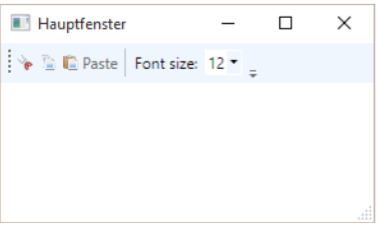
\includegraphics[scale=0.40]{Toolbar.png}
% \begin{lstlisting}[language=xml]
% <ToolBarTray DockPanel.Dock="Top">
%     <ToolBar>
%         <Button Command="Cut" ToolTip="...">
%             <Image Source="/media/clip_cut.png" Width="12" Height="12" />
%         </Button>
%     <Button Command="Copy" ToolTip="Copy selection to Windows Clipboard.">
%         <Image Source="/media/clip_copy.png" Width="12" Height="12" />
%     </Button>
%     <Button Command="Paste" ToolTip="Paste from Windows Clipboard.">
%         <StackPanel Orientation="Horizontal">
%             <Image Source="/media/clip_paste.png" Width="12" Height="12" />
%             <TextBlock Margin="3,0,0,0">Paste</TextBlock>
%         </StackPanel>
%     </Button>
%     <Separator />
%     <Label>Font size:</Label>
%     <ComboBox>
%         <ComboBoxItem>10</ComboBoxItem>
%         <ComboBoxItem IsSelected="True">12</ComboBoxItem>
%         <ComboBoxItem>14</ComboBoxItem>
%         <ComboBoxItem>16</ComboBoxItem>
%     </ComboBox>
%     </ToolBar>
% </ToolBarTray>
% \end{lstlisting}
% \paragraph{Ribbon} Das Ribbon ist seit Office 2007 bekannt und ist seither immer stärker verbreitet. 
% \begin{lstlisting}[language=xml]
% <Ribbon Name="Ribbon">
%     <Ribbon.ApplicationMenu>
%         <RibbonApplicationMenu SmallImageSource="media/home.png">
%             <RibbonApplicationMenuItem Header="Hello _Ribbon"
%                 Name="MenuItem1"
%                 ImageSource="media/home.png"/>
%         </RibbonApplicationMenu>
%     </Ribbon.ApplicationMenu>
%     <RibbonTab x:Name="HomeTab" Header="Start">
%         <RibbonGroup x:Name="Clipboard" Header="Clipboard">
%             <RibbonButton x:Name="Button1" Label="Paste"
%                 LargeImageSource="media/clip_paste.png" />
%             <RibbonButton x:Name="Button2" Label="Cut"
%                 SmallImageSource="media/clip_cut.png" />
%             <RibbonButton x:Name="Button3" Label="Copy"
%                 SmallImageSource="media/clip_copy.png" />
%         </RibbonGroup>
%     </RibbonTab>
% </Ribbon>
% \end{lstlisting}
% 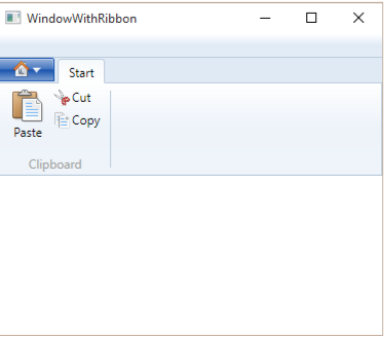
\includegraphics[scale=0.35]{Ribbon.png}
% \section{Commands} bieten eine Alternative zum Event. Commands müssen nicht abgefangen und behandelt werden, sie werden durch die Control selbst aufgerufen. Es ist eine standartisierte Ausführung eines Befehls und ermöglicht die Wiederverwendung derselben Aktion. Eine Command-Methode muss \verb+RoutedUICommand+ als Rückgabetyp haben und statisch sein.
% \begin{lstlisting}
% public static RoutedUICommand MyCutCommand = new RoutedUICommand(
%     "Ausschneiden",
%     "MyCut",
%     typeOf(WindowWithToolbar)
% );
% \end{lstlisting}
% Der \verb+RoutedUICommand+ nimmt auch noch einen 4. Paramter entgegen, in dem man \verb+InputGestures+ entweder einzeln oder als \verb+InputGestureCollection+ mitgeben kann.
% \begin{lstlisting}[language=xml]
% <MenuItem Header="_Cut" InputGestureText="CTRL + X" Command="local:WindowWithToolbar.MyCutCommand" />
% \end{lstlisting}
% Commands können auch an Event-Handler gebunden werden und Shortcuts definiert werden.
% \begin{lstlisting}[language=xml]
% <!-- Binding an Event -->
% <Window.CommandBindings>
%     <CommandBinding Command="local:WindowWithToolbar.MyCutCommand" Executed="MyCutCommand_Executed" />
% </Window.CommandBindings>
% <!-- Shortcut definieren -->
% <Window.InputBindings>
%     <KeyBinding Key="X" Modifiers="Control" Command="local:WindowWithToolbar.MyCutCommand" />
% </Window.InputBindings>
% \end{lstlisting}
% Im Code-Behind kann dann wie gewohnt ein Handler definiert werden.
% \begin{lstlisting}
% public void MyCutCommand_Executed(object sender, ExecutedRoutedEventArgs e){ ... }
% \end{lstlisting}
% \section{Automated UI Testing}
% 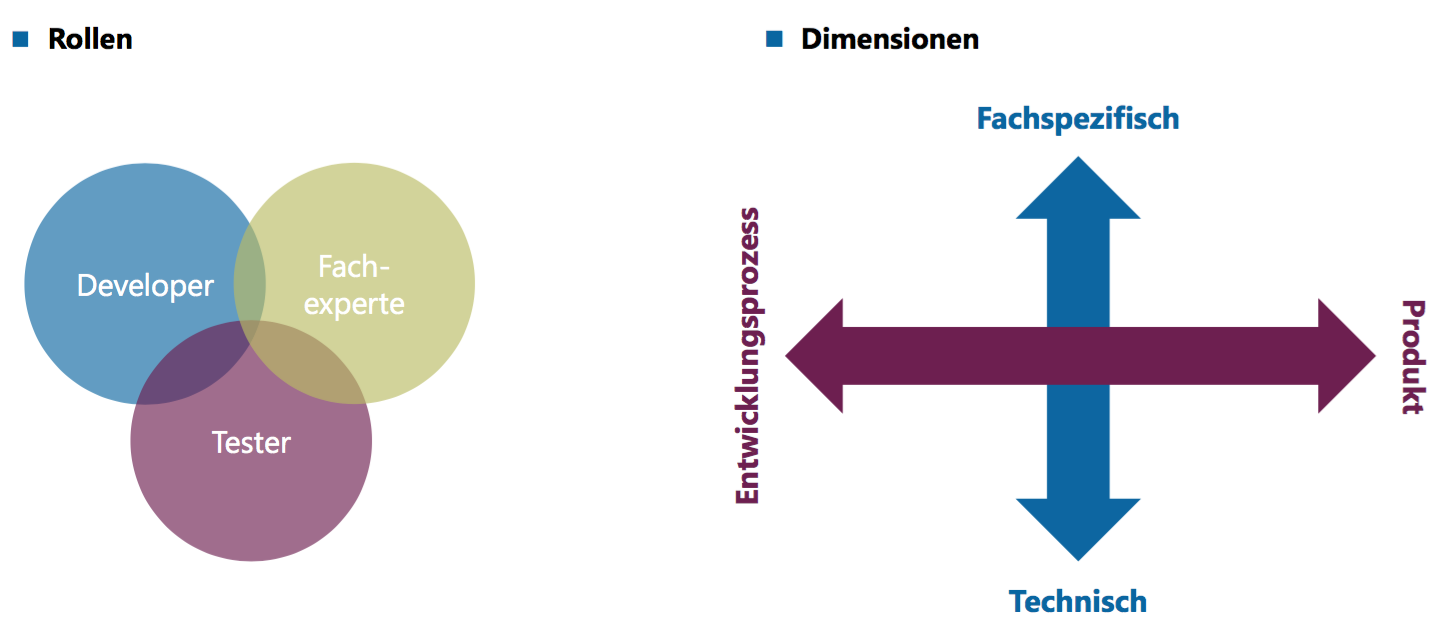
\includegraphics[scale=0.25]{Testing1.png}
% 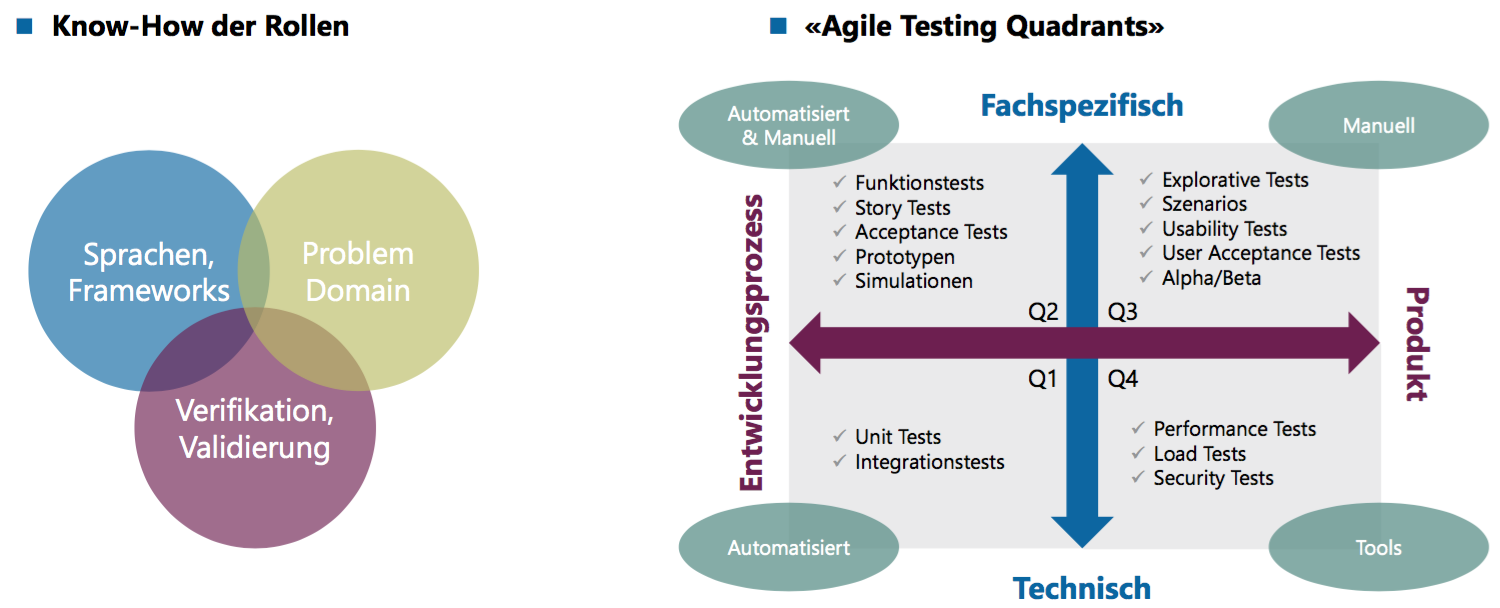
\includegraphics[scale=0.25]{Testing2.png}
% 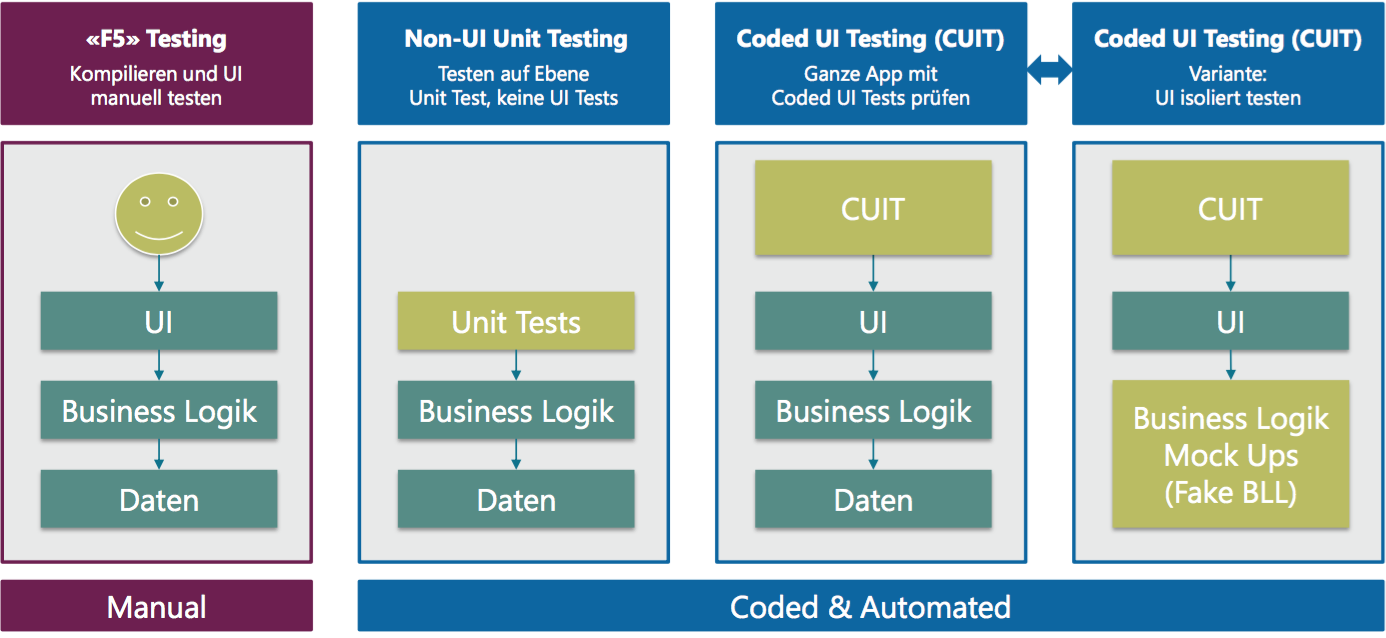
\includegraphics[scale=0.25]{Testing3.png} \\
% Es gibt 4 Varianten UIs zu testen. Das \textbf{Non-UI Unit Testing} Test auf Code Ebene (normale Unit-Tests) und führt keine UI-Tests durch. Das \textbf{Coded UI Testing (CUIT)} testet die ganze App mit Coded UI Tests. Diese Variante kann man auch mit isolierten UI Komponenten durchführen, welche dann aber Fake Komponenten benötigen (die 4. Variante ist das F5-Testing, der Benutzer testet die App gleich selbst).
% \subsection{TestStack}
% Der TestStack ist eine Sammlung von OpenSource Projekten um Tests in .NET Projekten zu automatisieren. Dazu gehört das \textbf{TestStack.White} Framework. Es ist ein CUIT-FW für WPF und basiert auf Microsofts UI Automation Framework. \\
% Als Vorbereitung muss man eine Testklasse erstellen.
% \begin{lstlisting}
% [TestClass]
% public class MyUiTest
% {
%     [TestMethod]
%     public void MyUiTestMethod(){ ... }
% }
% \end{lstlisting}
% Danach muss man das Verzeichnis mit der WPF App Assembly festlegen. Dies kann dann als Read-Only Property in der Testklasse hinzugefügt werden.
% \begin{lstlisting}
% // Directory in which tests are running
% public string BaseDir => Path.GetDirectoryName(Assembly.GetExecutingAssembly().Location);
% // System under test
% public string SutPath => Path.Combine(BaseDir, ${nameof(MenusAndCommands)}.exe);
% //$
% \end{lstlisting}
% Nun kann man die Tests entwickeln. \\
% Zuerst neues Application Objekt aus dem WPF App Assembly erstellen:
% \begin{lstlisting}
% var app = Application.Launch(SutPath);
% \end{lstlisting}
% Die Variable enthät ein UI-Automatisierungsobjekt des Typs \verb+TestStack.Whie.Application+.
% Danach kann man die Fenster abrufen:
% \begin{lstlisting}
% // Mit Fenstertitel abrufen
% var window = app.GetWindow("Hauptfenster", InitializeOption.NoCache);
% // Aus Liste der Fenster abrufen
% var window = app.GetWindows.First();
% // Anhand der ID(Name-Attribut) abrufen
% var window = app.getWindow(SearchCriteria.ByAutomationId"(Win1"), InitializeOption.NoCache);
% \end{lstlisting}
% Die Variable \verb+window+ enthäht nun ein UI-Automatisierungsobjekt des Typs \verb+TestStack.White.UIItems.WindoItems.Window+.\\
% Danach muss man die Controls abrufen:
% \begin{lstlisting}
% // Anhand Beschriftung abrufen
% var button = window.Get<Button>(SearchCriteria.ByText("Speichern"));
% // Anhand ID(Name-Attribut) abrufen
% var button window.Get<Button>("SaveButton");
% \end{lstlisting}
% Die Variable \verb+button+ enthält nun ein UI-Automatisierungsobjekt des Typs \verb+TestStack.White.UIItems.Button+.\\
% Schlussendlich können Aktionen ausgeführt werden:
% \begin{lstlisting}
% Assert.AreEqual("Speichern", button.Text);
% button.Click();
% Assert.AreEqual("Gespeichert!", button.Text);
% \end{lstlisting}
% \begin{lstlisting}
% var input = window.Get<TextBox>("NameInput");
% Assert.IsTrue(string.IsNullOrEmpty(input.Text));
% var newText = "You've been hacked!";
% input.Text = newText;
% Assert.AreEqual(newText, input.Text);
% \end{lstlisting}
% Schlussendlich muss die App noch mittels \verb+app.Close()+ beendet werden.\\
% Mit \verb+Desktop.CaptureScreenshot()+ erhält man ein Bitmap Objekt mit einem Bild des aktuellen Bildschirms.
% \begin{lstlisting}
% var screenshot = Desktop.CaptureScreenshot();
% var path = System.IO.Path.Combine(BaseDir, "screenshot.png");
% screenshot.Save(path, ImageFormant.Png);
% \end{lstlisting}

